\documentclass{beamer}

\usepackage[utf8]{inputenc}
%\usepackage{default}

\usetheme{Berlin}

\title{Imagerie Médicale}
\subtitle{Ingénierie d'une application}
\author{Jérôme Velut}
\date{04/12/2013}

\begin{document}

\frame{\titlepage}

\section*{Sommaire}
\begin{frame}{Sommaire}
  \tableofcontents[hideallsubsections]
\end{frame}

\section{Imagerie médicale}
\subsection{Bref historique}
\begin{frame}{Médecine nucléaire}
\begin{columns}[T]
 \begin{column}{0.5\textwidth}
 \centering
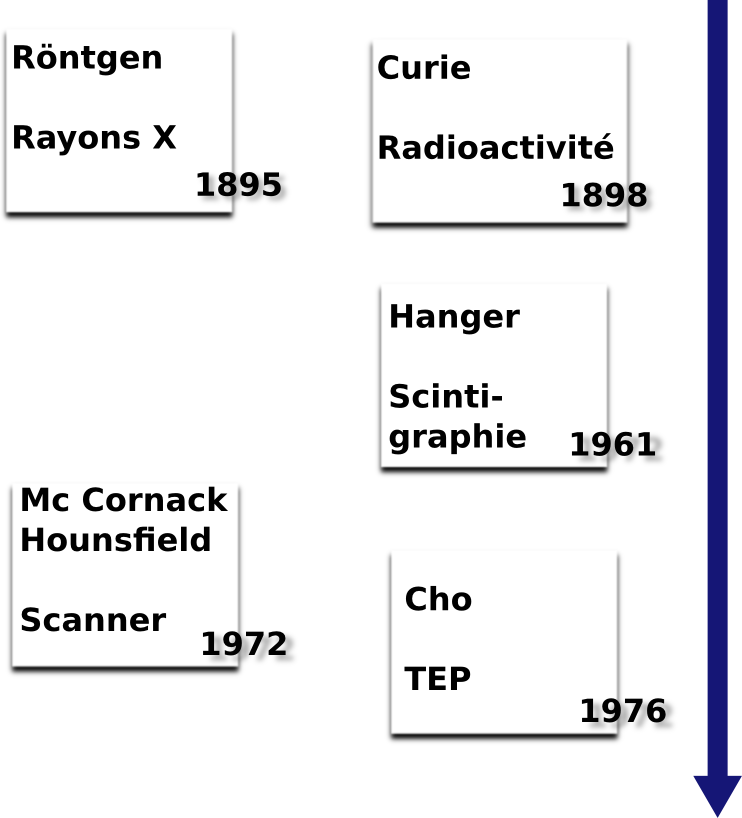
\includegraphics[height=0.7\textheight]{images/historique_radio.png}
 \end{column}
 \begin{column}{0.5\textwidth}
\begin{itemize}
 \item Médecine nucléaire: imageries, traitements par rayonnement ionisant
 \item Applications industrielles également
 \item Effets sur la santé
\end{itemize}
 \end{column}
\end{columns}
\end{frame}
\begin{frame}{Médecine nucléaire}
\begin{columns}[T]
 \begin{column}{0.5\textwidth}
 \centering
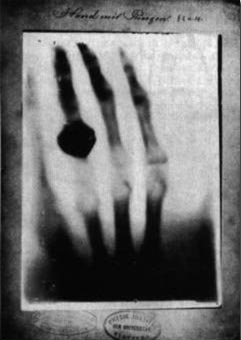
\includegraphics[height=0.7\textheight]{images/main_roentgen.jpg}\\
Première radiographie
 \end{column}
 \begin{column}{0.5\textwidth}
 \centering
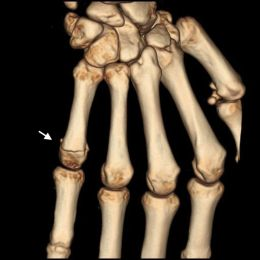
\includegraphics[height=0.5\textheight]{images/main_TDM.jpg}\\
Scanner haute résolution (fracture)
 \end{column}
\end{columns}
\end{frame}
\begin{frame}{Résonance magnétique}
\begin{columns}[T]
 \begin{column}{0.5\textwidth}
 \centering
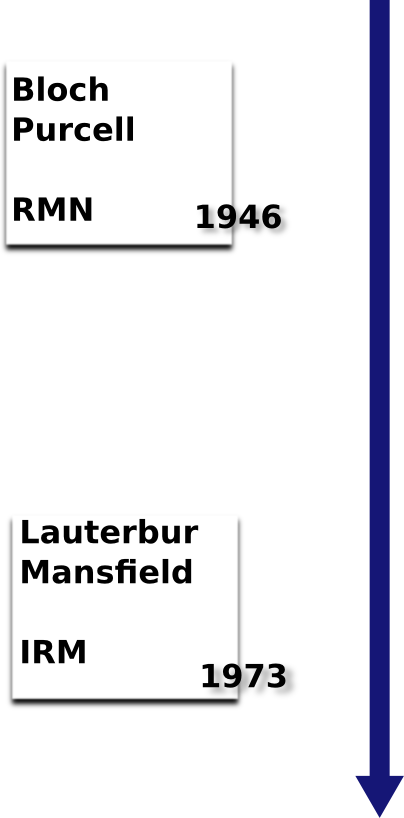
\includegraphics[height=0.7\textheight]{images/historique_rmn.png}
 \end{column}
 \begin{column}{0.5\textwidth}
\begin{itemize}
 \item Emission d'une onde radiofréquence par les noyaux placés dans un champ magnétique
 \item Spectroscopie RMN : observation de différents isotopes
 \item IRM: observation de l'hydrogène
\end{itemize}
 \end{column}
\end{columns} 
\end{frame}
\begin{frame}{Résonance magnétique}
\begin{columns}[T]
 \begin{column}{0.5\textwidth}
 \centering
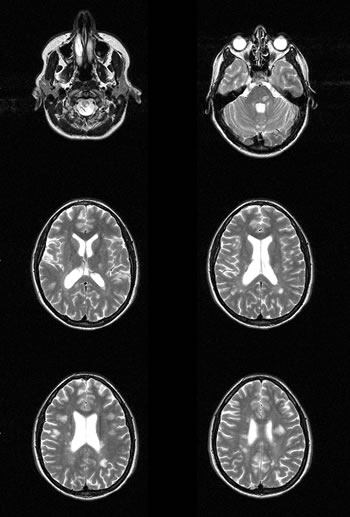
\includegraphics[height=0.6\textheight]{images/irm_t2.jpg}\\
IRM pondération T1
 \end{column}
 \begin{column}{0.5\textwidth}
 \centering
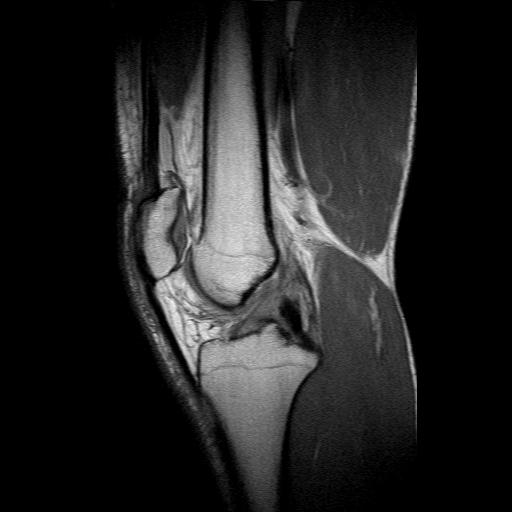
\includegraphics[height=0.6\textheight]{images/IRM_genou_sag_2.png}\\
IRM pondération T2
 \end{column}
\end{columns} 
\end{frame}

\begin{frame}{Ultrasons}
 
\end{frame}

\subsection{Méthodes de diagnostic}
\begin{frame}{Diagnostic}
 
\end{frame}

\begin{frame}{Anatomique}
 
\end{frame}

\begin{frame}{Fonctionnel}
 
\end{frame}

\subsection{Thérapie guidée par l'image}
\begin{frame}{Planification}
 
\end{frame}

\begin{frame}{Couplages}
 
\end{frame}

\subsection{Thérapie par ultrasons focalisés de haute intensité}
\begin{frame}{Indications}
 
\end{frame}

\begin{frame}{Technologie}
 
\end{frame}

\begin{frame}{Apport de l'IRM}
 
\end{frame}


\section{Recalage d'images}
\subsection{Objectifs}
\begin{frame}{Mise en correspondance}
 
\end{frame}

\subsection{Méthode}
\begin{frame}{Vue globale}
 
\end{frame}
\begin{frame}{Métrique}
 
\end{frame}

\subsection{Recalage multimodal}
\begin{frame}{Information mutuelle}
 
\end{frame}
\begin{frame}{Limitation}
 
\end{frame}

\subsection{Recalage basé modèle}
\begin{frame}{Entrées}
 
\end{frame}
\begin{frame}{Similarité}
 
\end{frame}

\section{Autres applications}
\subsection{Stabilisation de vidéos}
\begin{frame}{Stabilisation}
 
\end{frame}

\subsection{Segmentation basée sur des atlas}
\begin{frame}{Segmentation}
 
\end{frame}
\subsection{Interpolation}
\begin{frame}{Interpolation}
 
\end{frame}


\end{document}
